\documentclass[11pt]{article}
\usepackage[utf8]{inputenc}
\usepackage[T1]{fontenc}
\usepackage{amsmath}
\usepackage{amsfonts}
\usepackage{amssymb}
\usepackage[version=4]{mhchem}
\usepackage{stmaryrd}
\usepackage{hyperref}
\hypersetup{colorlinks=true, linkcolor=blue, filecolor=magenta, urlcolor=cyan,}
\urlstyle{same}
\usepackage{graphicx}
\usepackage[export]{adjustbox}
\graphicspath{ {./images/} }

\begin{document}
Long-hold Buyout Funds

PE GPs are adding a new strategy to their traditional buy-to-sell strategy. Several large PE GPs have launched long-hold fund structures with holding periods roughly double compared to the traditional PE hold period of 3 to 5 years. Blackstone Group LP, CVC Capital Partners Ltd., Carlyle Group LP, and KKR \& Co. are among the firms that have set up such vehicles and some have even raised their second fund. Long-hold private equity funds (long-hold PE funds) have a stated fund life of 15 years or longer, with some even exceeding 20 years. This contrasts with the traditional PE fund with a typical fund life 10 years with multiple one-year extensions. It is estimated that long-hold PE funds accounted for about $4.4 \%$ of the buyout and growth capital raised by funds over $\$ 1$ billion since $2015 .^{1}$ S\&P Global Intelligence (2019). Long-term fund strategies gaining ground in private equity. Extracted from: \href{https://www.spglobal.com/marketintelligence/en/news-insights/latest-newsheadlines/long-term-fund-strategies-gaining-ground-in-private-equity-50645295}{https://www.spglobal.com/marketintelligence/en/news-insights/latest-newsheadlines/long-term-fund-strategies-gaining-ground-in-private-equity-50645295}

Long-hold PE funds could improve some of the shortcomings in the traditional PE fund model. First, GPs are sometimes forced to sell because of the expiration of fund life instead of a business rationale or market conditions. Second, GPs who are raising a new fund may be under pressure to sell strong performers prematurely to demonstrate a verifiable track record or to provide distributions to existing LPs for reinvestment. Third, instead of holding good assets for as long as possible, GPs are sometimes incentivized to exit in a short time frame to post a high IRR and crystalize their carry.

Another consideration is the trend of increased secondary buyouts (SBOs), where PE firms are increasingly selling companies to each other. For a large LP who often has stakes in funds offered by numerous general partners, they are potentially subject to LP overlap where investors find themselves on both the buying and selling side of a SBO transaction. Degeorge, Martin, Phalippao (2015)2 Degeorge, Francois, Jens Martin, and Ludovic Phalippao (2015), On Secondary Buyouts. In Swiss Finance Institute Research Paper No. 13-48. \href{https://papers.ssrn.com/sol3/Delivery.cfm/SSRN}{https://papers.ssrn.com/sol3/Delivery.cfm/SSRN} ID2620560 code375762.pdf?abstractid =2329202\&mirid=1 concluded that in such LP overlap, the SBO does not generate extra transaction costs despite the LP being represented on both sides of the transactions. This is because the LP would have incurred those transaction costs anyway if the transaction involved a third party. However, they highlighted that SBO transactions between firms with complementary skill sets generate significantly higher returns for buyers than SBOs between firms with similar skill sets. Therefore a large LP, who has a higher chance of LP overlap, may be better off investing with a smaller number of buyout GPs instead of many GPs with similar skillset and strategy. They could consider diversifying their GP base when new GPs can offer complementary skill sets or strategies in the buyout space. Investing in long-hold buyout fund allows LPs to invest for the long term with a smaller set of GPs, and allows LPs to not worry about reinvestment as capital will be continuously deployed for a longer period.

The performance of long-hold PE funds is yet to be seen. While some managers successfully raised a second series of long-hold funds, there are not many realizations to support the performance of long-hold PE funds. According to an analysis by Bain (2018) ${ }^{3}$ Source: Bain \& Company (2018): Spotlight on Long-Hold Funds: Opening Up New Horizons. Bain \& Company publication. \href{https://www.bain.com/contentassets/9f88dfb08f024461b99987698c44d843/bain}{https://www.bain.com/contentassets/9f88dfb08f024461b99987698c44d843/bain} brief spotlight on long=

hold\_funds.pdf long-hold PE funds could potentially outperform traditional PE funds on an after-tax basis, provided that the fund's portfolio companies perform in an equivalent period during the long-hold period. The outperformance is driven by eliminating transaction fees, deferring capital gains, and keeping the fund fully invested. The exhibit Modeled Performance of Long-Hold PE Funds versus Traditional PE Funds shows the analysis where the modeled return of a long-hold PE fund that sells an investment after 24 years compared to a traditional PE fund selling four successive companies over that period. Such a comparison is difficult because it may not be an apples-to-apples comparison since the risk profile would be quite different between a long-hold fund and a PE fund.

\begin{center}
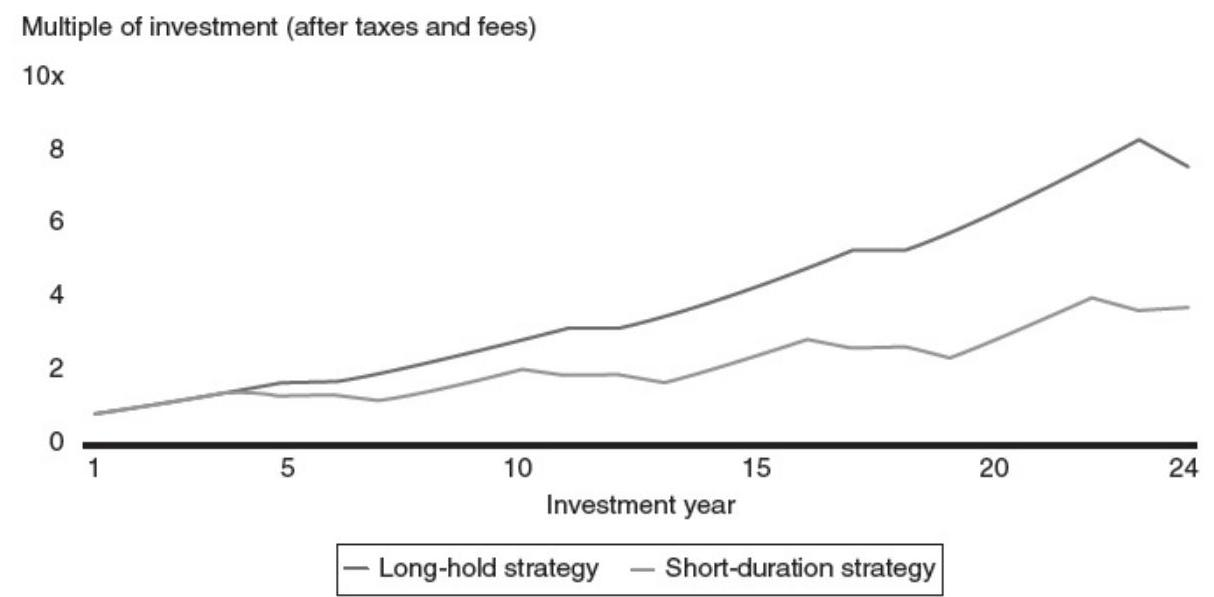
\includegraphics[max width=\textwidth]{2024_04_10_d21380c1d129a5bbd875g-2}
\end{center}

\section*{Modeled Performance of Long-Hold PE Funds versus Traditional PE Funds}
Source: Bain \& Company (2018): Spotlight on Long-Hold Funds: Opening Up New Horizons. Bain \& Company publication, page 4, Figure 1. \href{https://www.bain.com/contentassets/9f88dfb08f024461b99987698c44d843/bain}{https://www.bain.com/contentassets/9f88dfb08f024461b99987698c44d843/bain} brief spotlight on long-hold funds.pdf

Long-hold PE funds are a nascent concept, thus there are no established standard terms, and some funds are customized for specific LPs. Generally, there are two main types of long-hold PE funds:

\begin{enumerate}
  \item "Core" buyout funds target portfolio companies with lower risk and lower return. For example, the long-hold fund could have a 15-year life span and target a lower IRR of $12 \%$ to $14 \%$ while charging lower fees.

  \item Long-hold buyout funds target risk/return profiles, as well as fees, in line with traditional buyout funds.

\end{enumerate}

Other notable differences with traditional PE funds include:

\begin{itemize}
  \item Carry: For long-hold funds, where exits may happen 15 years later, there are various approaches to the calculation of incentive fees. Fees may be calculated on revaluation from year 7 onwards, or replace carry with stock options for listed PE firms.
\end{itemize}

It is important to point out that not all investments are suited to the long-hold strategy. Distressed, turnaround, and cyclical plays are some examples. Businesses that may be disrupted by new technologies may also not be suitable for such strategy. The ideal portfolio companies for long-hold funds are high-quality companies\\
that are well positioned to compound earnings over a long timeframe and across business cycles. These may be businesses taking market share over a long period, or have long tailwinds based on macro factors such as demographics.

Investors looking for a potentially lower-risk strategy to match their multi-decade investment horizon may find long-hold PE funds worth considering. However, investors who are using PE primarily for return enhancement and expect a high level of distributions in 5 to 10 years may not find long-dated PE funds suitable. It is important for investors who are considering long-hold PE funds to weigh the potential benefits and drawbacks. The potential benefits of long-hold PE funds include:

\begin{itemize}
  \item Lower transaction costs. These include legal, advisory, and due diligence costs, which are incurred each time a company is bought and sold. This will happen less frequently in a long-hold PE fund.
  \item Fully invested capital over longer periods and with less time waiting to be reinvested. This means that LPs will expend due diligence effort on fewer PE funds due to the lower turnover between funds.
  \item Deferred taxation of capital gains allowing capital to compound over time.
  \item Greater flexibility on exit timing.
\end{itemize}

The potential drawbacks include:

\begin{itemize}
  \item Increased illiquidity. Unlike the PE secondary market, where LPs can increase liquidity by selling a fund stake early, long-hold PE funds are essentially the opposite, as they prolong the hold period beyond that of the traditional PE fund.
  \item Lower IRR return profile. While long-hold PE funds may enjoy higher after tax and after fee returns on both multiple and dollar bases, the IRR return profile is lower than the traditional PE fund because of the longer time horizon.
  \item Issues around incentivizing investment professionals. With the longer fund life, there is a delay in realizations, which delays carried interest. In addition, the longer fund life may increase key person risk as the longer fund life makes it more likely that personnel may retire or change firms
  \item Limited scope for value-add. The typical target companies for long-hold PE funds are stable, mature, and fundamentally good businesses. It is unclear how much growth and operational improvements can be added to these companies after they reach a mature stage of development. Furthermore, it is likely GPs would have to pay up for these high-quality companies and would need to ensure there is further scope to grow the business to ensure a profitable exit.
\end{itemize}

\end{document}